\state{Central limit theorem}{
	Consider a one-dimensional system consisting of a large number of non-interacting particles on a circle of circumference $L$.  Assume that the positions of the particles are independent random variables
(i.r.v.) uniformly distributed on the circle.
}



%
%	1.1
%

\prob{}{ \label{prob1.1}
	Find the probability $\pN(t, \alp)$ of observing exactly $\alp N$ of the $N$ particles in a fixed arc of length $t L$, where $t, \alp \in [0, 1]$.  (For $\alp = 0$ this is called \emph{gap} (or \emph{void}) \emph{formation probability}.)
	
	Find the leading behavior of the result in the limit $N \to \infty$ with $t, \alp$ fixed.  (You may use the Stirling formula $n! \approx n^n e^{-n} \sqrt{2\pi n}$.  A good sanity check for the answer is that $\int_0^1 \pN(t, \alp) \dd{\alp}$ evaluated with a computer should be 1.)
	
	Make a plot of this leading term as a function of $\alp \in [0, 1]$ for $N = 100$ and $t = 0.1$, overlaid with the exact discrete distribution.  Describe any qualitative changes in the plot as $N$ and $t$ change, and whether the asymptotic approximation breaks down anywhere.
}

\sol{
	Consider a single particle $i$ on the circle.  The probability of observing it in an arc of length $t L$ is $p = t$.  This is equivalent to a Bernoulli trial with failure probability $q = 1 - p = 1 - t$.  The binomial distribution gives the probability of obtaining exactly $k$ successes out of $N$ such trials~\cite{Binomial}:
	\eqn{binomial}{
		P_p(k \,|\, N) = \mqty( N \\ k ) p^n q^{N - k}
		= \frac{N!}{k! \,(N - k)!} p^k (1 - p)^{N - k}.
	}
	Assuming $k = \alp N$ is an integer, the probability of observing $\alp N$ of the $N$ particles in this arc is given by
	\eqn{exact}{
		\ans{ \pN(t, \alp) = \frac{N!}{(\alp N)! \,(N - \alp N)!} t^{\alp N} (1 - t)^{N - \alp N}. }
	}

	To find the leading behavior as $N \to \infty$, we use Stirling's approximation for $N!$, $(\alp N)!$, and $(N - \alp N)!$.  In doing so, we assume $N, \alp N, (1 - \alp) N \gg 1$.  This yields
	\aln{
		\pN(t, \alp) &\approx \frac{N^N e^{-N} \sqrt{2\pi N}}{(\alp N)^{\alp N} e^{-\alp N} \sqrt{2\pi \alp N} (N - \alp N)^{N - \alp N} e^{\alp N - N} \sqrt{2\pi (N - \alp N)}} t^{\alp N} (1 - t)^{N - \alp N} \notag \\
%		&= \frac{N^N e^{-N} \sqrt{2\pi N}}{\alp^{\alp N} N^{\alp N} (N - \alp N)^{N - \alp N} e^{-N} 2 \pi \sqrt{\alp N (N - \alp N)}} t^{\alp N} (1 - t)^{N - \alp N} \notag \\
		&= \frac{N^{N - \alp N}}{\alp^{\alp N} N^{N - \alp N} (1 - \alp)^{N - \alp N} \sqrt{2 \pi \alp (N - \alp N)}} t^{\alp N} (1 - t)^{N - \alp N} \notag \\
%		&= \frac{t^{\alp N} (1 - t)^{N - \alp N}}{\alp^{\alp N} (1 - \alp)^{N - \alp N} \sqrt{2 \pi \alp (N - \alp N)}} \notag \\
		&= \ans{
			\frac{1}{\sqrt{2 \pi \alp (1 - \alp) N}} \left( \frac{t}{\alp} \right)^{\alp N} \left( \frac{1 - t}{1 - \alp} \right)^{N - \alp N}.
		} \label{approx}
	}
	A plot comparing this approximation to the exact, discrete distribution is shown in Fig.~\ref{fig1.1} as a function of $\alp \in [0, 1]$ for $N = 100$ and $t = 0.1$.  Both distributions becomes broader and shorter as $t$ is increased to $0.5$, and then narrower and taller as $t$ is increased from there.  The area under the curve becomes smaller as $N$ increases, although its shape does not change.  This makes sense because $\pN(t, \alp)$ as a function of $\alp$ is not a PDF; the PDF is $P_t(k | N)$ as a function of $k = \alp N$.  The area under the curve of $\pN(t, \alp)$ is $1/N$.
	
	For $t \lapp 0.2$ and $t \gapp 0.8$, the approximate distribution has a slightly sharper and higher peak than the discrete distribution.  This is slightly visible in Fig.~\ref{fig1.1}  This discrepancy becomes more pronounced as $N$ decreases.  For $N \lapp 20$, a discrepancy near the peak is visible even for $t = 0.5$.  The approximation visibly diverges as $\alp \to 0$ for $t \lapp 0.2$ and as $\alp \to 1$ for $t \gapp 0.8$.  This effect becomes more pronounced as $N$ decreases.  For $N \lapp 25$, this divergence overtakes the expected behavior of the discrete distribution, and so the approximation becomes poor.
	
	\fig{fig1.1}{
		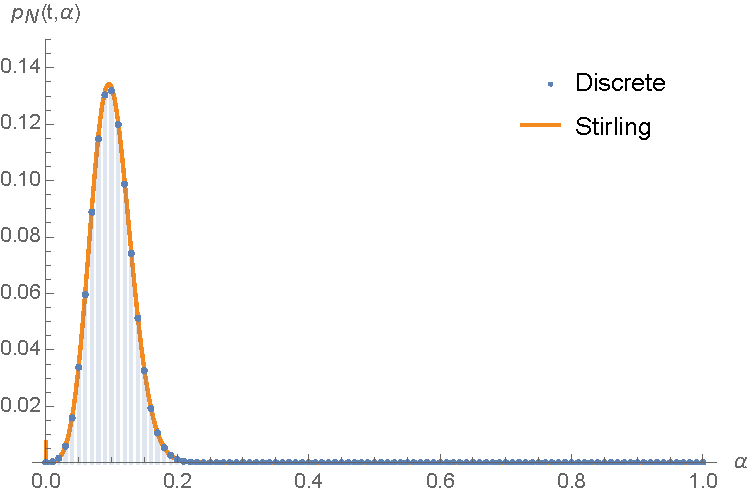
\includegraphics{Figure1-1}
		\caption{Comparison of the discrete expression~(Eq.~\refeq{exact}, blue) and Stirling's approximation to~(Eq.~\refeq{approx}, orange) $\pN(t, \alp)$ as functions of $\alp \in [0, 1]$ for $N = 100$ and $t = 0.1$.}
	}
}



%
%	1.2
%

\prob{}{
	In the large-$N$ limit, find the average number $k$ (or the fraction $\alp = k / N$) of particles in the arc of length $t L$ for a given $t \in [0, 1]$, and the fluctuation (variance) of this number, using the Central Limit Theorem.  Plot the corresponding Gaussian distribution over $\alp \in [0, 1]$ and add it to the previous plot.  How good is this approximation?
}

\sol{
	The mean of the binomial distribution is $\mu = N p$, and the variance is $\sig^2 = N p q$~\cite{Binomial}.  Thus, the mean and variance of Eq.~\refeq{exact} are,
	\al{
		\ans{\muB} &\ans{= Nt}, &
		\ans{\sigB^2} &\ans{= N t (1 - t)},
	}
	which correspond to the average number of particles in $t L$ and the variance of that number, respectively.
	
	By the Central Limit Theorem, we may approximate Eq.~\refeq{exact} by a Gaussian distribution~\cite{Gaussian}
	\eq{
		P(x) = \frac{e^{-(x - \mu)^2 / (2 \sig^2)}}{\sig \sqrt{2\pi}},
	}
	with mean $\muG = \muB = Nt$ and standard deviation $\sigG = \sigB / \sqrt{N} = \sqrt{t (1 - t)}$~\cite{CLT}.  (The factor of $1/N$ in the variance is necessary because $\pN(t, \alp)$ is not normalized.)  Since $x$ is equivalent to $k =  \alp N$, this gives us the Gaussian distribution
	\eqn{CLT}{
		\pN(t, \alp) \approx \frac{e^{-N^2 (\alp - t)^2 / 2 t (1 - t)}}{\sqrt{2\pi t (1 - t)}}.
	}
	This distribution is shown overlaid with the discrete distribution and Stirling's approximation in Fig.~\ref{fig1.2}.  The CLT approximation, being Gaussian, is perfectly symmetrical for all $t$, unlike the discrete function and Stirling's approximation, which both become more skew as $t \to 0$ and $t \to 1$.  This effect is visible in Fig.~\ref{fig1.2}.  The CLT is a worse approximation than Stirling in these cases, except when $N$ is very large~($\gapp 1000$).  In this limit, the quality of both approximations is about the same.  However, the CLT approximation has no singularities, making it a better approximation when $\alp, t \approx 0$ and $\alp, t \approx 1$.
	
	\fig{fig1.2}{
		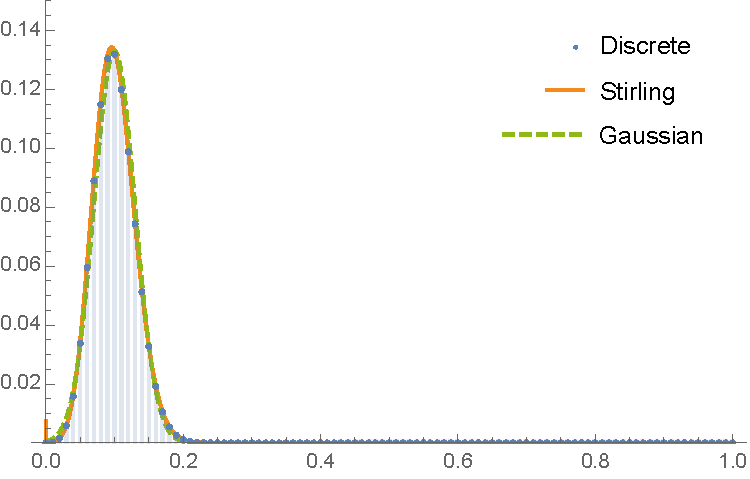
\includegraphics{Figure1-2}
		\caption{Comparison of the discrete expression~(Eq.~\refeq{exact}, blue), Stirling's approximation to~(Eq.~\refeq{approx}, orange), and CLT approximation to~(Eq.~\refeq{CLT}, green) $\pN(t, \alp)$ as functions of $\alp \in [0, 1]$ for $N = 100$ and $t = 0.1$.}
	}
}



%
%	1.3
%

\prob{}{
	Defining the number density $n(x) = \sumiN \del(x - \xii)$, compute
the two-point correlation function
	\al{
		C(x, y) &= \ev{\deln(x) \cdot \deln(y)}, &
		\deln(x) &= n(x) - \evn,
	}
which describes the fluctuations of the density.
}

\sol{
	Firstly, the mean $\evn$ is found by
	\eq{
		\evn = \frac{1}{L} \intoL n(x) \dx
		= \frac{1}{L} \intoL \sumiN \del(x - \xii) \dx
		= \frac{1}{L} \sumiN \intoL \del(x - \xii) \dx
		= \frac{N}{L}.
	}
	Then
	\al{
		C(x, y) &= \frac{1}{L^2} \intoL \intoL \deln(x) \, \deln(y) \dx \dy
		= \frac{1}{L^2} \intoL \left( \sumiN \del(x - \xii) - \frac{N}{L} \right) \dx \intoL \left( \sumiN \del(y - \yii) - \frac{N}{L} \right) \dy \\
		&= \frac{1}{L^2} \left( \sumiN \intoL \del(x - \xii) \dx - \frac{N}{L} \intoL \dx \right) \left( \sumiN \intoL \del(y - \yii) \dy - \frac{N}{L} \intoL \dy \right) \\
		&= \frac{1}{L^2} \left( N - \frac{N}{L} \bigg[ x \bigg]_0^L \right) \left( N - \frac{N}{L} \bigg[ y \bigg]_0^L \right) \\
		&= \ans{0}.
	}
	This result suggests that the positions of different particles on the circles are not correlated~\cite[p.~360]{Landau}.  This is sensible since the locations of the particles are random and uniformly distributed, and the particles do not interact with one another.
}